\documentclass[border=2pt]{standalone}
\usepackage{diagrams}
\usetikzlibrary{patterns,angles,quotes,arrows.meta,math,calc}
\usepackage{amsmath}
\begin{document}
  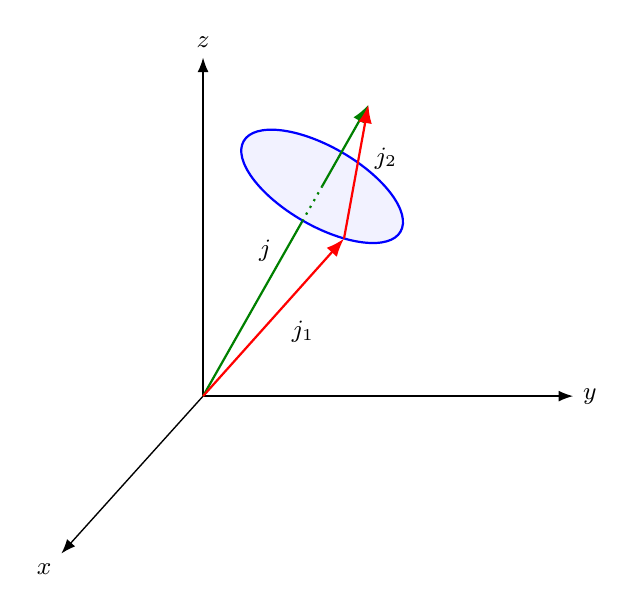
\begin{tikzpicture}[>=Latex,line width=0.5pt,font=\small]
  % --- coordinate axes ---
  \coordinate (O) at (0,0);
  \draw[->] (O) -- (0,4.3)    node[above]{$z$};
  \draw[->] (O) -- (4.7,0)    node[right]{$y$};
  \draw[->] (O) -- (-1.8,-2.0) node[below left]{$x$};
  % --- vectors: j = j_1 + j_2 ---
  \coordinate (J)  at (2.1,3.7);            % tip of resultant j
  \coordinate (M)  at ($(O)!0.72!(J)$);     % circle centre, on the j axis
  \coordinate (P)  at (1.79,2.0);           % tip of j_1 (a point on the circle)
  % resultant j (drawn first so the circle can occlude it)
  \draw[thick,color=green!50!black] (O) -- (M);
  % the circle of possible j_1 endpoints (perp. to j), in perspective
  \draw[thick,color=blue,rotate around={-30:(M)},fill=blue!5] (M) ellipse (1.15 and 0.5);
  \draw[thick,dotted,color=green!50!black] ($(O)!0.60!(J)$) -- (M);    % hidden portion behind the circle
  \draw[thick,->,color=green!50!black] (M) -- (J);
  % j_1 and j_2
  \draw[thick,->,color=red] (O) -- (P);
  \draw[thick,->,color=red] (P) -- (J);
  % labels
  \node[left]       at ($(O)!0.5!(J)+(-0.06,0)$) {$j$};
  \node[below right=0.5pt] at ($(O)!0.55!(P)$)          {$j_{1}$};
  \node[right]      at ($(P)!0.6!(J)+(0.08,0)$)   {$j_{2}$};
  \end{tikzpicture}
\end{document}